%杨舒云的实验报告编辑界面,使用了Huanyu Shi,2019级的模板,杨舒云在此拜谢ORZ!

%!TEX program = xelatex
\documentclass[dvipsnames, svgnames,a4paper,11pt]{article}
% ----------------------------------------------------- 
%	加边框的命令
%	参考:https://tex.stackexchange.com/questions/531559/how-to-add-the-page-border-for-first-two-pages-in-latex
\usepackage{tikz}
\usetikzlibrary{calc}
\usepackage{eso-pic}
\AddToShipoutPictureBG{%
\begin{tikzpicture}[overlay,remember picture]
\draw[line width=0.6pt] % 边框粗细
    ($ (current page.north west) + (0.6cm,-0.6cm) $)
    rectangle
    ($ (current page.south east) + (-0.6cm,0.6cm) $); % 边框位置
\end{tikzpicture}}


\usepackage{xcolor}
\definecolor{c1}{HTML}{086173} % 目录颜色 原版为2752C9 紫灰色535AAA 蓝紫色0B0DB7 深蓝色070F94 湖绿色219394 松石灰绿086173
\definecolor{c2}{HTML}{E20129} % 引用颜色 原版\definecolor{c2}{RGB}{190,20,83} 橙色F24729

\usepackage{ctex}
\usepackage[top=28mm,bottom=28mm,left=15mm,right=15mm]{geometry}
\usepackage{hyperref} 
\hypersetup{
	colorlinks,
	linktoc = section, % 超链接位置,选项有section, page, all
	linkcolor = c1, % linkcolor 目录颜色
	citecolor = c1  % citecolor 引用颜色
}
\usepackage{amsmath,enumerate,multirow,float}
\usepackage{tabularx}
\usepackage{tabu}
\usepackage{subfig}
\usepackage{fancyhdr}
\usepackage{graphicx}
\usepackage{wrapfig}  
\usepackage{physics}
\usepackage{appendix}
\usepackage{amsfonts}

%
\usepackage{tcolorbox}
\tcbuselibrary{skins,breakable}
\newtcolorbox{tbox}[2][]{
    colframe=black!70!,
    breakable,
    enhanced,
	boxrule =0.5pt,
    title = {#2},
    fonttitle = \large\kaishu\bfseries,
	drop fuzzy shadow,
    #1
}
\newtcolorbox[auto counter,number within=section]{question}[1][]{
  top=2pt,bottom=2pt,arc=1mm,
  boxrule=0.5pt,
%   frame hidden,
  breakable,
  enhanced, %跨页后不会显示下边框
  coltitle=c1!80!gray,
  colframe=c1,
  colback=c1!3!white,
  drop fuzzy shadow,
  title={思考题~\thetcbcounter:\quad},
  fonttitle=\bfseries,
  attach title to upper,
  #1
}

% ---------------------------------------------------------------------
%	利用cleveref改变引用格式,\cref是引用命令
\usepackage{cleveref}
\crefformat{figure}{#2{\textcolor{c2}{Figure #1}}#3} % 图片的引用格式
\crefformat{equation}{#2{(\textcolor{c2}{#1})}#3} % 公式的引用格式
\crefformat{table}{#2{\textcolor{c2}{Table #1}}#3} % 表格的引用格式


% ---------------------------------------------------------------------
%	页眉页脚设置
\fancypagestyle{plain}{\pagestyle{fancy}}
\pagestyle{fancy}
\lhead{\kaishu 中山大学物理与天文学院\uppercase\expandafter{\romannumeral1}} % 左边页眉,学院 + 课程
\rhead{\kaishu 杨舒云的实验报告} % 右边页眉,实验报告标题
\cfoot{\thepage} % 页脚,中间添加页码


% ---------------------------------------------------------------------
%	对目录、章节标题的设置
\renewcommand{\contentsname}{\centerline{\huge 目录}}
\usepackage{titlesec}
\usepackage{titletoc}
% \titleformat{章节}[形状]{格式}{标题序号}{序号与标题间距}{标题前命令}[标题后命令]
\titleformat{\section}{\centering\LARGE\songti}{}{1em}{}

% ---------------------------------------------------------------------
%   listing代码环境设置
\usepackage{listings}
\lstloadlanguages{python}
\lstdefinestyle{pythonstyle}{
backgroundcolor=\color{gray!5},
language=python,
frameround=tftt,
frame=shadowbox, 
keepspaces=true,
breaklines,
columns=spaceflexible,                   
basicstyle=\ttfamily\small, % 基本文本设置,字体为teletype,大小为scriptsize
keywordstyle=[1]\color{c1}\bfseries, 
keywordstyle=[2]\color{Red!70!black},   
stringstyle=\color{Purple},       
showstringspaces=false,
commentstyle=\ttfamily\scriptsize\color{green!40!black},%注释文本设置,字体为sf,大小为smaller
tabsize=2,
morekeywords={as},
morekeywords=[2]{np, plt, sp},
numbers=left, % 代码行数
numberstyle=\it\tiny\color{gray}, % 代码行数的数字字体设置
stepnumber=1,
rulesepcolor=\color{gray!30!white}
}




% ---------------------------------------------------------------------
%	其他设置
\def\degree{${}^{\circ}$} % 角度
\graphicspath{{./images/}} % 插入图片的相对路径
\allowdisplaybreaks[4]  %允许公式跨页 
\usepackage{lipsum}
\usepackage{adjustbox}
%\usepackage{mathrsfs} % 字体
\captionsetup[figure]{name=Figure} % 图片形式
\captionsetup[table]{name=Table} % 表格形式
\usepackage{enumitem}
\usepackage{tabularray}  %绘制表格时可以更加方便添加框线
\usepackage{xcolor} %添加更多文本颜色

\begin{document}
	
	
	
	% 实验报告封面	
	
	% 顶栏
	\begin{table}
		\renewcommand\arraystretch{1.7}
		\begin{tabularx}{\textwidth}{
				|>{\centering}X|>{\centering}X|>{\centering}X
				|>{\centering}X|>{\centering}X|>{\centering\arraybackslash}X|}
			\hline
			\multicolumn{2}{|c|}{预习报告}&\multicolumn{2}{c|}{实验记录与分析}&\multicolumn{2}{c|}{总成绩}\\
			\hline
			\LARGE30 & & \LARGE50 & & \LARGE80 & \\
			\hline
		\end{tabularx}
	\end{table}
	% ---
	
	% 信息栏
	\begin{table}
		\renewcommand\arraystretch{1.7}
		\begin{tabularx}{\textwidth}{|X|X|X|X|}
			\hline
			年级、专业: & 2022级 物理学 &组号: & 实验班2\\
			\hline
			姓名: & 杨舒云  & 学号: & 22344020\\
			\hline
			实验时间: & 2024/3/21 & 教师签名: & \\
			\hline
		\end{tabularx}
	\end{table}
	% ---
	
	% 大标题
	\begin{center}
		\LARGE Lab2-3 \quad 全息照相实验
	\end{center}
	% ---
	
	% 注意事项
	
	% 基本
	\textbf{【实验报告注意事项】}
	\begin{enumerate}[label=\arabic*., leftmargin=*]
		\item 实验报告由两部分组成:
		\begin{enumerate}[label=\arabic*), leftmargin=*]
			\item 预习报告:课前认真研读\textbf{实验讲义},弄清实验原理;实验所需的仪器设备、用具及其使用、完成课前预习思考题;了解实验需要测量的物理量,并根据要求提前准备实验记录表格(可以参考实验报告模板,可以打印)。\textcolor{red}{\textbf{(30分)}}
			\item 实验记录与分析:认真、客观记录实验条件、实验过程中的现象以及数据。实验记录请用珠笔或者钢笔书写并签名(\textcolor{red}{\textbf{用铅笔记录的被认为无效}})。\textcolor{red}{\textbf{保持原始记录,包括写错删除部分,如因误记需要修改记录,必须按规范修改。}}(不得手记的值输入到电脑打印);离开前请实验教师检查记录并签名。\textcolor{red}{\textbf{(50分)}}
		\end{enumerate}
		
		\item \textcolor{red}{\textbf{本实验报告可提前打印出来,当场记录分析完成交给带实验的老师,课后无需再提交。若当场完成不了,则请课后完成,再扫描并通过seelight提交。}}
		
		\textcolor{red}{\textbf{注意:本文档已留出填写空间,若填写空间不够的话请提前规划留白,做到报告的美观}}
		\item 注意事项:
		\begin{enumerate}[label=\arabic*), leftmargin=*]
			\item 实验中\textcolor{red}{\textbf{避免激光器伤到眼睛}}
			\item 避免用手直接接触镜片的光学面
			\item 安装镜片时需在光学平台上尽量靠近台面的高度操作,以免失手跌落摔碎镜片
			\item 实验平台配件所用固定螺钉需拧紧,以免镜架晃动;但不可过紧,以免损坏
			\item 实验前需按仪器清单检查光学元件是否齐全,\textcolor{red}{\textbf{实验结束后按照顺序放回元件盒}}
			
		\end{enumerate}
	\end{enumerate}
	
	% 安全
	\textbf{【实验安全注意事项】}	
	\begin{enumerate}
		\item 光学元件要轻拿轻放,要注意保护光学表面,不要用手触摸表面;保持光学元件清洁,禁止用手或非擦镜纸擦拭;
		\item 注意激光安全,注意佩戴防护镜,避免激光直射入眼;
		\item 注意身体部位不要直接接触显影液、定影液等化学品,注意化学品和暗室规范使用;
		\item 实验过程中,注意尽量减少振动、噪声、气流干扰,并避免干扰他人实验。		
	\end{enumerate}
	
	% ---
	
	% 特别鸣谢
	\textbf{【特别鸣谢及模板说明】}	
	
	感谢2019级学长石寰宇为本实验报告提供\LaTeX 模板。\textcolor{red}{\textbf{由于原实验报告模板缺少实验编号,为方便在电脑上整理,故添加自命名编号Lab2-3}}
	% ---
	
	
	
	% 目录
	\clearpage
	\tableofcontents
	\clearpage
	% ---
	
	
	
	% 预习报告	
	
	% 小标题
	\setcounter{section}{0}
	\section{Lab2-2 全息照相实验 \quad\heiti 预习报告}
	% ---
	
	% 实验目的
	\subsection{实验目的}
	\begin{enumerate}
		\item 学习全息照相的基本原理和方法;
		\item 了解全息照相的主要特点;
		\item 学习全息照片的制作方法和技术;
		\item 学习观察全息照片的方法。
	\end{enumerate}
	% ---
	
	% 仪器用具
	\subsection{仪器用具}
	\begin{table}[htbp]
		\centering
		\renewcommand\arraystretch{1.6}
		% \setlength{\tabcolsep}{10mm}
		\begin{tabular}{p{0.05\textwidth}|p{0.20\textwidth}|p{0.05\textwidth}|p{0.5\textwidth}}
			\hline
			编号& 仪器用具名称 & 数量 &  主要参数(型号,测量范围,测量精度等) \\
			\hline
			1  & 防震光学平台 & 1  & --  \\
			2  & 氦氖激光器  & 1  & --  \\
			3  & 扩束透镜   & 1  & --  \\
			4  & 分束器    & 1  & --  \\
			5  & 反射镜    & 3  & --  \\
			6  & 全息干版   & 1  & --  \\
			7  & 显影液    & 1  & --  \\
			8  & 定影液    & 1  & --  \\
			9  & 暗房设备   & 1  & --  \\
			\hline
		\end{tabular}
	\end{table}
	% ---
	
	% 原理概述
	\subsection{原理概述}
	\begin{enumerate}
		\item 什么是全息图
		
		全息图是一种技术,最初由盖伯在1948年提出,目的是为了提高电子显微镜的图像质量,它能够详细记录光波前的振幅和相位信息。虽然盖伯的实验成功展示了全息图技术的基础原理,即记录和再现光波前,但因为当时没有强光源如激光器,所以成像质量很差。1962年,随着激光器的发明,利思和乌帕特尼克斯对盖伯的方法进行了改进,提出了离轴全息技术,解决了成像质量差的问题,并使得三维显示成为了研究的热点。到了1969年,本顿发明了彩虹全息图,这种技术可以在普通的白光下展示三维图像,并且相较于其他类型的全息图,它的处理和复制更为简单和方便。
		
		\begin{figure}[htbp]
			\centering
			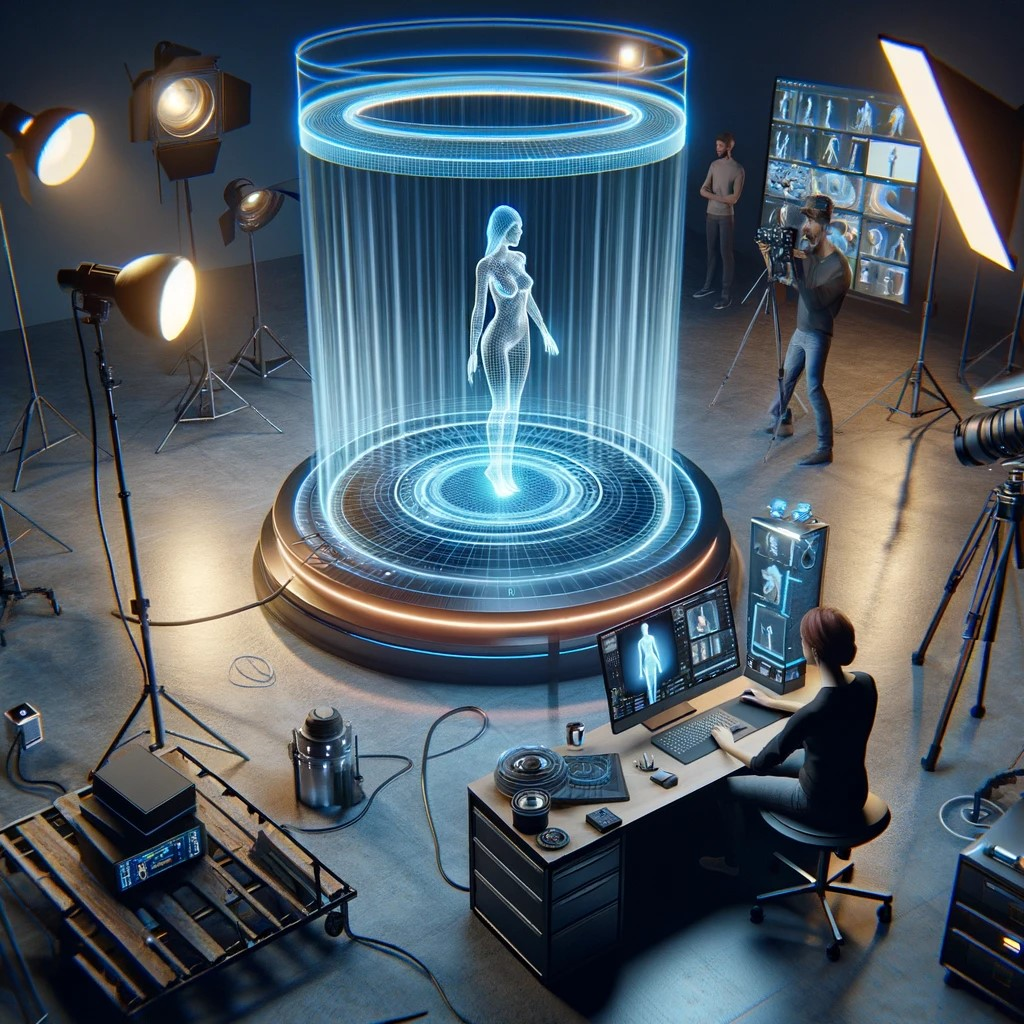
\includegraphics[width=0.4\textwidth]{Lab2_3Gra1.jpg}
			\caption{全息摄影概念图}
			\label{fig:fig1}
		\end{figure}
		
		\item 全息照相的特点
		
		全息照相是一种与传统照相技术在原理和方法上根本不同的技术。普通照相基于几何光学原理,通过透镜将物体的图像投影到平面上,记录的是图像点的光强或振幅,实现的是从三维到二维的转换,因此无法完全真实地再现物体。而全息照相利用光的干涉和衍射等物理现象,通过记录光波的振幅和相位信息,创造出包含物体完整信息的全息图。这种全息图不直接显示物体图像,而是通过细密的干涉条纹来编码物体信息,需要通过特定的光源照明才能重现原始的物体光波。
		
		全息照片具有几个独特的特点:
		\begin{enumerate}
			\item 在适当的照明条件下,全息照片可以重现与原始物光波相同的深度和视差,观看者可以从不同角度看到被遮挡的物体细节。
			\item 全息照片即使被切割成小片,也能重现整个场景。这是因为照片上的每一点都包含了整个场景的信息。但是,随着片段尺寸的减小,图像的分辨率也会下降。
			\item 全息照片可以通过接触式方法复制,复制品和原件一样,都能再现物体的正像,而且无论使用何种照明,再现的图像与原物体的对比度非常接近。
			\item 如果将全息照片绕不同的轴线旋转180°,它会产生不同的图像倒置效果,但绕着与全息图平面垂直的轴线旋转180°则不会引起像的倒转。
			\item 全息照片还能在同一张底片上通过连续曝光技术重叠多个图像,每个图像都能独立显示,而不会相互干扰。
		\end{enumerate}
		
		\item 全息照相的物理原理
		
		全息照相是一种利用光的相干性来创建图像的技术。它包括两个主要步骤:首先,使用一束光(称为参考光)和照射到物体上的另一束光(称为物光)在一个特定的介质上形成一个复杂的干涉模式,这个干涉模式被称为全息图。其次,通过适当的照明技术,可以从这个全息图中再现出物体的三维图像。这个过程基于双光束干涉场的计算,是一种广义上的光学成像理论。
		
		在全息照相中,一台激光器产生相干光,这束光被一个分束器分成两部分:一部分直接照射物体并形成物光,另一部分作为参考光。这两束光在记录介质上以一定角度相遇并干涉,从而形成全息图。由于记录介质通常只能记录光的强度(或振幅),物光的相位信息是通过与参考光干涉并转换为振幅信息记录下来的。
		
		简化地说,可以通过考虑从点光源发出的球面波的干涉来理解全息图的基本特性。因为任何广泛的光源或被照射物体都可以看作是许多点光源的集合,而平面波则可以视为来自无限远处点源的球面波。这样的处理使得我们对全息图的理解具有普遍性。
		
		\begin{enumerate}
			\item 全息照相记录的信号
			
			\begin{figure}[htbp]
				\centering
				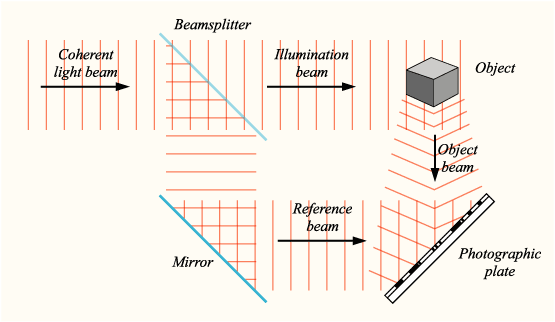
\includegraphics[width=0.7\textwidth]{Lab2_3Gra2.png}
				\caption{全息照相记录的信号(参考文献[1])}
				\label{fig:fig2}
			\end{figure}
			
			全息照相技术中,记录的信号涉及物体(物点)和记录介质(如全息图平面)之间的光波传播。设想一个简单的场景,物点P位于一定位置,而记录介质(比如全息图)位于另一个平面上,两者之间的空间关系通过特定的坐标来描述。全息照相过程中,从物点P发出的光波(物光)和从另一个点R发出的参考光波在记录介质上相遇并产生干涉,形成光强分布模式。这个模式不仅包括两波各自的光强,还包括它们相互作用的结果,即干涉项。
			
			干涉项的核心是物光和参考光之间的相位差,这导致记录介质上形成按照余弦规律变化的干涉条纹。这些条纹的形成基于物光和参考光到达记录介质上某点的光程差,即两者从发出点到达记录点的路径长度差。由于光波的振幅和相位信息都蕴含在这些干涉条纹中,通过记录这些条纹,全息图便能够保存下来物光的完整信息,包括其振幅和相位。
			
			简而言之,当物光和参考光在记录介质上相遇并产生干涉时,它们的相互作用形成了特定的光强分布模式。这个分布既包括各自的光强,也包括由于相位差而产生的干涉条纹。这些条纹记录了从物点发出的光波的全貌,包含了光波的振幅和相位信息。因此,全息照相能够通过记录这些干涉模式,保存并再现出物体的三维形态和特征。
			
			\begin{figure}[htbp]
				\centering
				\subfloat[]{
					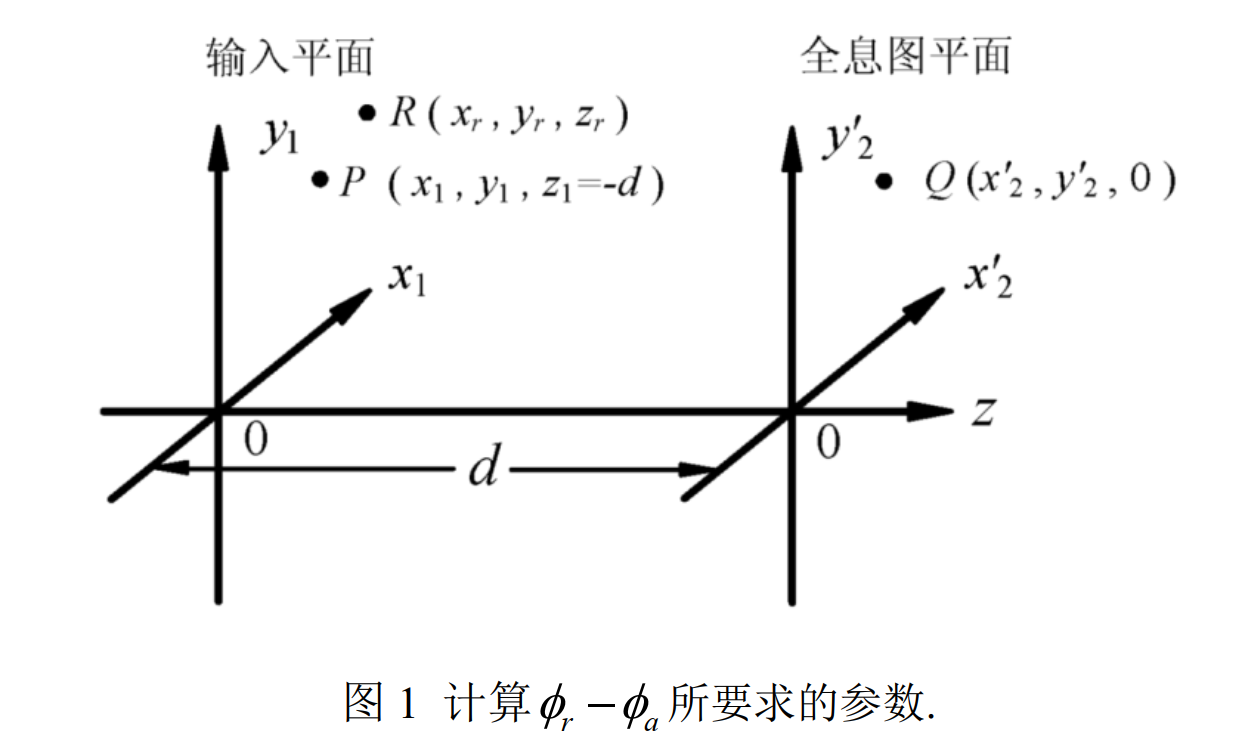
\includegraphics[width=0.4\textwidth]{Lab2_3Gra3.png}
				}
				\subfloat[]{
					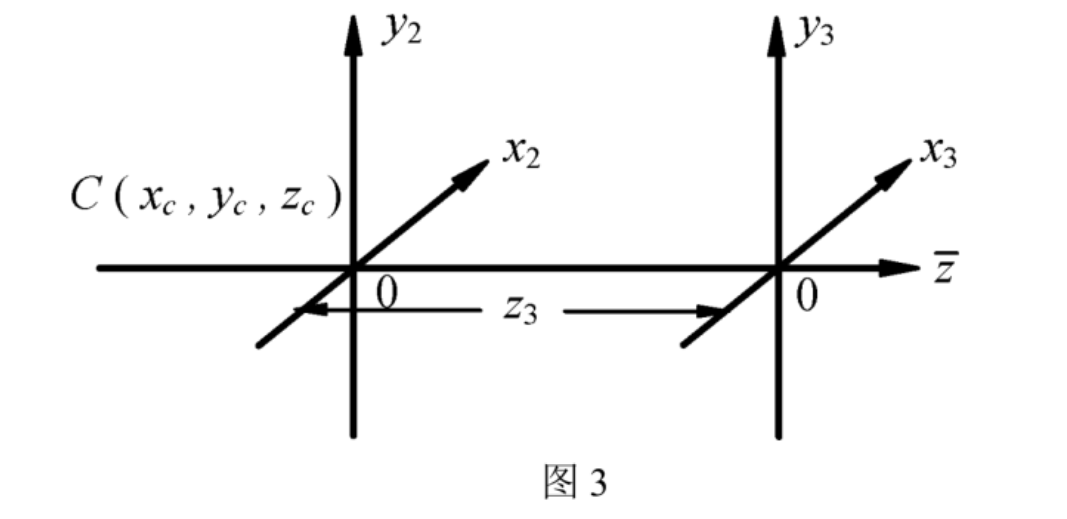
\includegraphics[width=0.4\textwidth]{Lab2_3Gra4.png}
				}
				\caption{讲义上的示意图}
				\label{fig:fig3}			
			\end{figure}
			
			以下是全息照相记录信号的公式,描述了物体波\(O(r,t)\)和参考波\(R(r,t)\)的复振幅表达式,以及它们在全息照相介质上产生的光强分布\(I(r,t)\)。
			
			物体波和参考波的表达式为:
			\[
			\begin{aligned}
				& O(r,t)=A_0(r)e^{i(\phi_0-\omega t)}\\
				& R(r,t)=A_R(r)e^{i(\phi_R-\omega t)}
			\end{aligned}
			\]
			这里,\(A_0(r)\)和\(A_R(r)\)分别是物体波和参考波在位置\(r\)的振幅;\(\phi_0\)和\(\phi_R\)是它们的初始相位;\(\omega\)是光波的角频率;\(t\)是时间。
			
			当物体波和参考波在全息照相介质上相遇时,它们的叠加光强\(I(r,t)\)可以表示为:
			\[
			I(r,t) = (O+R)^2 = |O|^2 + |R|^2 + 2|O||R|\cos(\phi_0-\phi_R)
			\]
			这里,\(|O|\)和\(|R|\)分别是物体波和参考波的振幅;\(\cos(\phi_0-\phi_R)\)表示由两波相位差引起的干涉项。
			
			\item 波前重现
			
			波前重现在全息照相中是通过将记录介质(如照相干版或胶片)上记录的全息图进行曝光、冲洗后,使得曝光过程中的光强变化转换为记录介质上显影振幅透射率的变化。记录介质的透射率与记录时物光与参考光形成的干涉图样密切相关,这种干涉图样反映了物体的光波振幅和相位信息。再现过程中,可以通过改变全息图的大小或使用不同波长的光来照明全息图,从而重建物体的光波。
			
			\begin{figure}[htbp]
				\centering
				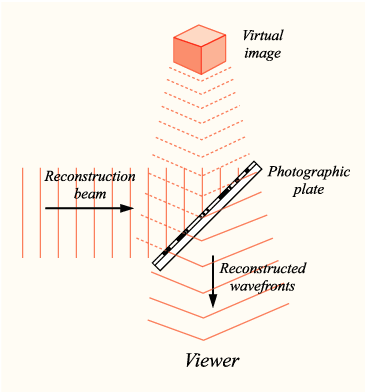
\includegraphics[width=0.4\textwidth]{Lab2_3Gra5.png}
				\caption{波前重现(参考文献[1])}
				\label{fig:fig5}
			\end{figure}
			
			波前重现的公式描述了如何通过照明已记录的全息图来重现物体的光波。设全息图的透射率为\(\tau(x,y)\),则有:
			\[
			\tau(x,y)=\tau_0+\beta I(x,y)=\tau_0+\beta\left[|O|^2+|R|^2+R^*|O|+R|O|^*\right] \quad (\beta<0)
			\]
			这里,\(\tau_0\)是未曝光部分的透射率;\(\beta\)是与材料相关的常数;\(R^*\)和\(O^*\)分别是参考波和物体波的复共轭。
			
			再现波\(A_{rec}(r,t)\)可以通过用参考波\(R(r,t)\)或其共轭波\(R^*(r,t)\)照明全息图获得。如果用参考波照明,再现波为:
			\[
			A_{rec}(r,t)=R(r,t)\tau(r)=R\left[\tau_0+\beta\left(|O|^2+|R|^2\right)\right]+\beta RR^*O+\beta R^2O^*
			\]
			如果用共轭参考波照明,再现波为:
			\[
			A_{rec}(r,t)=R^*(r,t)\tau(r)=R^*\left[\tau_0+\beta\left(|O|^2+|R|^2\right)\right]+\beta (R^*)^2O+\beta |R|^2O^*
			\]
		\end{enumerate}
		
		\item 全息照相实验的实验条件
		
		在全息照相实验中,有两个主要条件需要特别注意:稳定性要求和光源相干性要求。
		
		\begin{figure}[htbp]
			\centering
			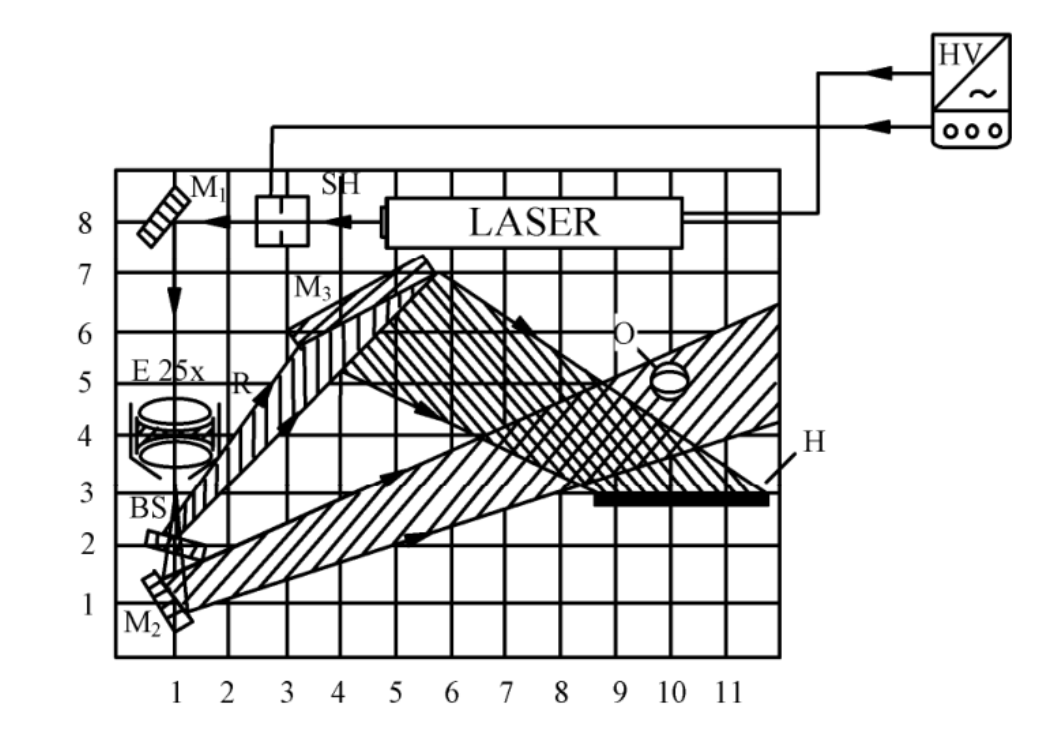
\includegraphics[width=0.7\textwidth]{Lab2_3Gra6.png}
			\caption{讲义上的实验光路图}
			\label{fig:fig6}
		\end{figure}
		
		\textbf{稳定性要求:} 由于全息照相记录的是非常细密的干涉条纹,任何微小的震动或扰动都可能导致干涉条纹模糊,甚至无法记录。例如,当使用波长为632.8纳米的激光并设定角度为30°时,干涉条纹的宽度大约为1.22微米。制作反射式全息图时,银层间隔甚至小于0.3微米。因此,物体在曝光时间内的移动超过波长的八分之一就足以使干涉条纹模糊。为了精确记录干涉条纹,曝光期间元件间的相对移动需要非常小,空气流动、声波、温度变化等因素也需要控制以避免引入振动。减少曝光时间可以降低外界影响,使用脉冲激光器能够拍摄运动中的物体全息图,但曝光时间的具体需求还受到光源强度和记录介质灵敏度的限制。
		
		\textbf{光源相干性要求:} 全息照相依赖于记录物体光波的振幅和相位的干涉方法,因此需要参考光束与物光束之间保持高度相干。在实验中,通常使用波长为632.8纳米的氦-氖激光器,尽管激光器的单色性很好,谱线宽度仍会影响相干长度。考虑到最不利的情况(如多普勒展宽为0.002纳米时),相干长度大约为20厘米。为了确保物光束与参考光束的相干,物光路与参考光路的光程需要尽量等长,被摄物体的景深也应在相干长度范围内。此外,还必须考虑空间相干性,选择单横模(TEM00)激光器,并确保景物大小在激光器的空间相干范围内。
	\end{enumerate}
	% ---
	
	
	
	% 实验前思考题
	\subsection{实验前思考题}
	
	% 思考题1
	\begin{question}
		实验中应该注意哪些影响因素才能够保证成功观察到全息再现图像?
	\end{question}
	为了成功观察到全息再现图像,实验中应该注意以下影响因素:
	
	\begin{enumerate}
		\item \textbf{稳定性要求:} 全息照相记录的是参考光束和物光束之间的干涉条纹,这些干涉条纹十分细密。因此,为了成功地记录干涉条纹,曝光期间,元件之间的相对位移应小于条纹间距的几分之一。此外,空气、声波和温度的变化也会引起元件的震动,或者使空气的流动密度不均匀而导致光程变化。因此,曝光期间应避免大声喧哗、敲门、吹风等,更不能碰到防震台。
		
		\item \textbf{光源相干性要求:} 全息照相是用干涉的方法记录物光波的振幅和位相,因此参考光束与物光束必须是相干的。为了保证物光束与参考光束相干,应使参考光路与物光路的光程接近相等。而被摄景物的景深也应该在相干长度之内。此外,对空间相干性的要求也是必不可少的。实验中使用的是单横模(TEM00)的激光器,景物的大小应在空间相干的范围内。
		
		\item \textbf{光路设置:} 确认光路中物光和参考光的光程差大致相等,物光和参考光夹角适当(30-50°),物光和参考光光强比适宜(3:1-5:1)。这有助于保证干涉条纹的质量,从而成功记录并再现全息图像。
		
		\item \textbf{显影和处理过程:} 全息片经过显影、停影、定影、水漂及晾干等步骤后才能观察再现。显影时间应与曝光量、显影液的浓度及温度等情况加以综合考虑,以避免显影过度或不足,影响全息图的质量。
	\end{enumerate}
	
	综上所述,为了保证成功观察到全息再现图像,需要控制实验的稳定性,确保光源的相干性,正确设置光路,并严格控制显影和处理过程。这些因素共同作用,确保全息图的质量,从而能够成功再现出物体的三维图像。
	
	
	% 思考题2
	\begin{question}
		物光和参考光的光程差应保持在什么范围?为什么?
	\end{question}
	\begin{itemize}
		\item 物光和参考光的光程差应保持在相干长度的范围内,以确保两者能够有效地相干干涉。相干长度是指光源发出的光波能够保持相干状态的最大传播距离,这与光源的单色性有关。激光器由于其良好的单色性和相干性,相干长度通常较长,可达数十米甚至更长。但在全息照相中,由于实验条件和干涉记录介质的限制,物光和参考光的光程差通常需要控制在较小的范围内,比如几厘米到几十厘米之间,这样可以确保在全息图记录过程中,两束光能够有效干涉,从而记录下物体的三维信息。
		
		\item 在实验讲义中提到,使用的He-Ne激光器的波长为632.8nm,但没有直接提及光程差的具体数值范围。然而,讲义中强调了为了保证物光束与参考光束相干,应使参考光路与物光路的光程接近相等,以及考虑到激光器的相干长度通常为几十厘米的量级,因此物光和参考光的光程差应尽量控制在这个量级内,以保证良好的干涉效果。此外,讲义还指出,被摄景物的景深也应该在相干长度之内,进一步强调了控制光程差以保持光波相干性的重要性。
		
		\item 如果光程差过大,超出了相干长度,那么物光和参考光之间的相干性会下降,这将导致干涉条纹质量下降,影响全息图的质量和再现图像的清晰度。因此,实验中应该尽量确保物光和参考光的光程差不会超过光源的相干长度,并通过调整实验光路来控制光程差,以获得高质量的全息图。
	\end{itemize}
	
	% ---
	
	
	
	% 实验记录	
	\clearpage
	
	% 顶栏
	\begin{table}
		\renewcommand\arraystretch{1.7}
		\centering
		\begin{tabularx}{\textwidth}{|X|X|X|X|}
			\hline
			专业: & 物理学 & 年级: & 2022级 \\
			\hline
			姓名: & 杨舒云 & 学号: & 22344020\\
			\hline
			室温: &  & 实验地点: &  \\
			\hline
			学生签名:& 见\textbf{附件} & 评分: &\\
			\hline
			实验时间:& 2024/3/21 & 教师签名:&\\
			\hline
		\end{tabularx}
	\end{table}
	\section{Lab2-2 全息照相实验  \quad\heiti 实验记录}
	\subsection{实验内容、步骤、结果及讨论}\textcolor{ForestGreen}{(按照实验顺序依次}\textcolor{red}{简要记录}\textcolor{ForestGreen}{实验内容及步骤,)(空间不够,可自行加页)}\\
	\textcolor{red}{
		(注意: \\
		除了记录实验内容、步骤、参数外,还应记录:\\
		按比例绘制操作中实际摆放的实验光路(各元件间距离可通过直尺测量)\\
		记录光路中物光和参考光的光程差\\
		记录物光和参考光光强比\\
		记录是否可观察到再现图像\\
		)
	}
	
	
	
	
	%\subsection{实验数据记录}
	
	
	
	%\subsection{原始数据记录}
	
	\clearpage
	
	\newpage
	
	\null
	
	\newpage
	
	\null
	
	
	
	
	
	
	\newpage
	
	\subsection{实验过程中遇到的问题记录}
	
	\begin{enumerate}
		\item 
		\item 
		\item 
	\end{enumerate}
	\null
	
	
	
	
	
	
	
	% ---
	
	% 小标题
	\section{Lab2-2 全息照相实验  \quad\heiti 实验记录}
	% ---
	
	% 实验过程记录
	\subsection{实验内容、步骤与结果}
	
	%
	\subsubsection{操作步骤记录}
	\begin{enumerate}
		\item 
	\end{enumerate}	
	
	%
	\subsubsection{}
	\begin{enumerate}
		\item \begin{table}[h]
			\centering
			\caption{表格示例}
			\label{tab:tab1}
			\begin{tabular}{|c|c|c|c|c|c|}
				\hline
				组1/序号i & 1 & 2 & 3 & 4 & 5 \\
				$v_{1i}(m/s)$ & 1.26 & 1.08 & 1.00 & 0.75 & 0.38 \\
				$f_{1i}(Hz)$ & 40073 & 40127 & 40105 & 40088 & 40066 \\
				\hline
				组2/序号i & 1 & 2 & 3 & 4 & 5 \\
				$v_{2i}(m/s)$ & 1.21 & 1.06 & 0.99 & 0.52 & 0.57 \\
				$f_{2i}(Hz)$ & 40143 & 40125 & 40084 & 40080 & 40067 \\
				\hline
				组3/序号i & 1 & 2 & 3 & 4 & 5 \\
				$v_{3i}(m/s)$ & 1.15 & 0.98 & 0.78 & 0.59 & 0.36 \\
				$f_{3i}(Hz)$ & 40135 & 40115 & 40092 & 40070 & 40044 \\
				\hline
			\end{tabular}
		\end{table}		
	\end{enumerate}
	
	% ---
	
	% 原始数据
	\clearpage
	\subsection{原始数据记录}
	实验记录本上的原始数据见%\cref{}(签字)。
	
	实验台桌面整理见%\textbf{附件}部分(\cref{})。
	
	其它原始数据见%\cref{}。
	% ---
	
	% 问题记录
	\subsection{实验过程中遇到的问题记录}
	\begin{enumerate}
		\item 
	\end{enumerate}
	% ---
	
	
	
	% 分析与讨论	
	\clearpage
	
	% 顶栏
	\begin{table}
		\renewcommand\arraystretch{1.7}
		\begin{tabularx}{\textwidth}{|X|X|X|X|}
			\hline
			专业:& 物理学 &年级:& 2022级\\
			\hline
			姓名: & 杨舒云 & 学号:& 22344020\\
			\hline
			日期:& 2024// & 评分: &\\
			\hline
		\end{tabularx}
	\end{table}
	% ---
	
	% 小标题
	\section{Lab2-2 全息照相实验 \quad\heiti 分析与讨论}
	% ---
	
	% 数据处理
	\subsection{实验数据分析}
	
	%
	\subsubsection{}
	\begin{enumerate}
		\item 
	\end{enumerate}
	
	%
	\subsubsection{}
	\begin{enumerate}
		\item 
	\end{enumerate}
	
	%
	\subsubsection{}
	
	% ---
	
	% 实验后思考题
	\subsection{实验后思考题}
	
	%思考题1
	\begin{question}
		
	\end{question}
	
	% 思考题2
	\begin{question}
		
	\end{question}
	
	% 思考题3
	\begin{question}
		
	\end{question}
	
	% ---
	
	
	% 结语部分
	\clearpage
	
	% 小标题
	\section{Lab2-2 全息照相实验 \quad\heiti 结语}
	% ---
	
	% 总结、杂谈与致谢
	\subsection{总结、杂谈与致谢}
	\begin{enumerate}
		\item 
	\end{enumerate}
	% ---
	
	% 参考文献
	\subsection{参考文献}
	[1] 维基百科 https://zh.wikipedia.org
	
	[2] 沈韩.基础物理实验.——北京:科学出版社,2015.2 ISBN:978-7-03-043311-4
	
	% ---
	
	% 附件
	\subsection{附件}
	试验台桌面整理如%\cref{}所示。
	
	实验报告个人签名如\cref{fig:name}。
	
	\begin{figure}[htbp]
		\centering
		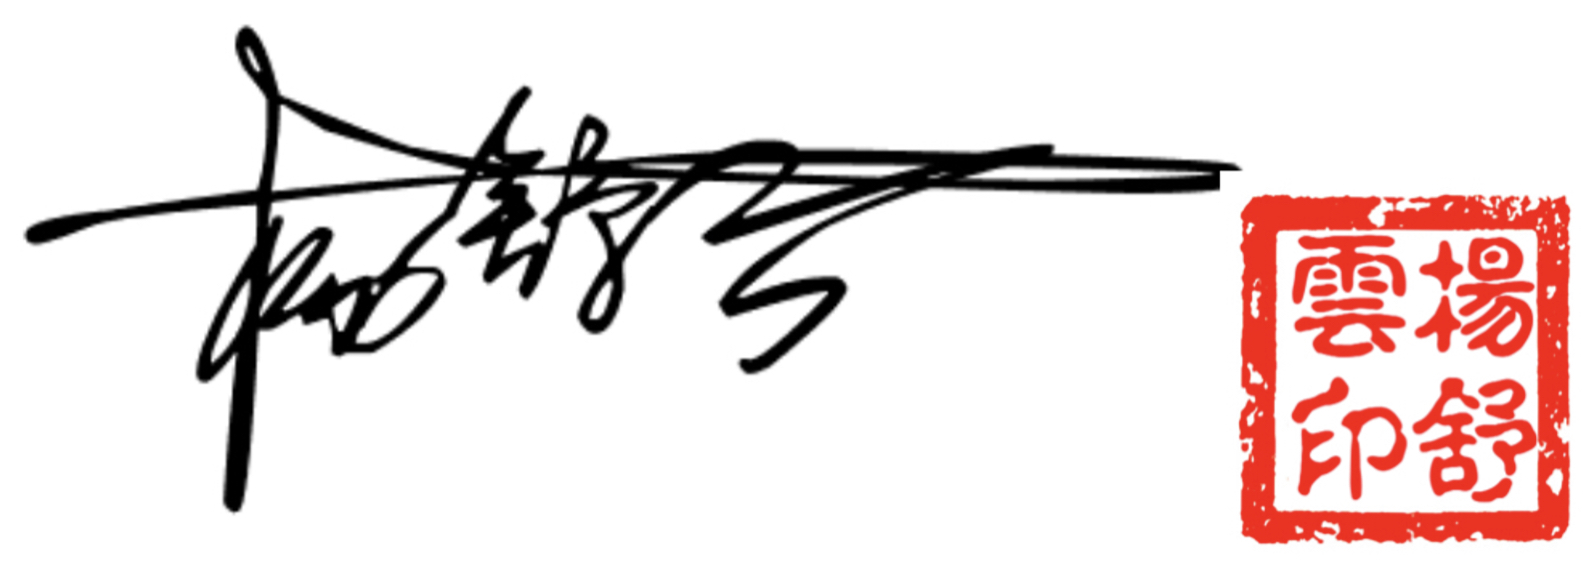
\includegraphics[width=0.7\textwidth]{name.png}
		\caption{个人签名}
		\label{fig:name}
	\end{figure}
	
	% ---
	
	相关代码已上传至Github。
	
	
	
\end{document}